\input{setup.tex}

% Режим шаблона (должен быть включен один из трех)
%\ВКРtrue
%\Практикаtrue
\Курсоваяtrue

\newcommand{\Дисциплина}{<<Проектирование и архитектура программных систем>>} % для курсовой
\newcommand{\КодСпециальности}{09.03.04} % Курсовая
\newcommand{\Специальность}{Программная инженерия} % Курсовая
\newcommand{\Тема}{Программа редактирования звуковых файлов} % ВКР Курсовая
\newcommand{\ТемаВтораяСтрока}{}
\newcommand{\ГдеПроводитсяПрактика}{Юго-Западном государственном университете} % для практики
\newcommand{\РуководительПрактПредпр}{Куркина А. В.} % для практики
\newcommand{\ДолжнРуководительПрактПредпр}{директор} % для практики
\newcommand{\РуководительПрактУнивер}{Чаплыгин А. А.} % для практики
\newcommand{\ДолжнРуководительПрактУнивер}{к.т.н. доцент} % для практики
\newcommand{\Автор}{А. Ю. Геворкян}
\newcommand{\АвторРод}{Геворкяна А. Ю.}
\newcommand{\АвторПолностьюРод}{Иванова Ивана Ивановича} % для практики
\newcommand{\Шифр}{21-06-0040}
\newcommand{\Курс}{4} % для практики
\newcommand{\Группа}{ПО-12б}
\newcommand{\Руководитель}{А. А. Чаплыгин} % для ВКР и курсовой
\newcommand{\Нормоконтроль}{А. А. Чаплыгин} % для ВКР
\newcommand{\ЗавКаф}{А. В. Малышев} % для ВКР
\newcommand{\ДатаПриказа}{2024~г.} % для ВКР
\newcommand{\НомерПриказа}{} % для ВКР
\newcommand{\СрокПредоставления}{2024~г.} % для ВКР, курсового
\begin{document}
\maketitle
\ifПрактика{}\else{
   \input{ЛистЗадания}
   \abstract{РЕФЕРАТ}

Объем работы равен \formbytotal{lastpage}{страниц}{е}{ам}{ам}. Работа содержит \formbytotal{figurecnt}{иллюстраци}{ю}{и}{й}, \formbytotal{tablecnt}{таблиц}{у}{ы}{} и \arabic{bibcount} библиографических источников. Количество приложений – 1. Фрагменты исходного кода представлены в приложении А.

Перечень ключевых слов: система, программа, редактор, интерфейс, пользователь, звук, аудиофайл, Python.

Объектом разработки является программа, представляющая собой набор иструментов для совершения операций над WAV аудиофайлами.

В процессе создания программы были выделены основные сущности путем создания информационных блоков, использованы классы и методы модулей, обеспечивающие работу с сущностями предметной области, а также корректную работу программы.

При разработке программы использовался язык программирования Python.

\selectlanguage{english}
\abstract{ABSTRACT}
  
The volume of work is \formbytotal{lastpage}{page}{}{s}{s}. The work contains \formbytotal{figurecnt}{illustration}{}{s}{s}, \formbytotal{tablecnt}{table}{}{s}{s} and \arabic{bibcount} bibliographic sources. The number of applications is 1. The program code is presented in annex A.

List of keywords: system, programm, editor, interface, use, sound, audiofile, Python.

The object of development is a program that is a set of tools for performing operations on WAV audio files.

In the process of creating the program, the main entities were identified by creating information blocks, classes and methods of modules were used to ensure work with the entities of the subject area, as well as the correct operation of the program.

When developing the program, the Python programming language was used.
\selectlanguage{russian}
}\fi
\tableofcontents
\section*{ОБОЗНАЧЕНИЯ И СОКРАЩЕНИЯ}

WAV (Waveform Audio File Format) -- формат файла-контейнера для хранения записи оцифрованного аудиопотока, подвид RIFF. Как правило, используется для хранения несжатого звука в импульсно-кодовой модуляции.

UML (Unified Modelling Language) -- язык графического описания для объектного моделирования в области разработки программного обеспечения.

\ifПрактика{}\else{\section*{ВВЕДЕНИЕ}
\addcontentsline{toc}{section}{ВВЕДЕНИЕ}

В современном мире аудиозаписи играют значительную роль в нашей повседневной жизни. От музыки, которую мы слушаем на наших устройствах, до голоса, который мы слышим на радио и телевидении, аудио является неотъемлемой частью нашего существования. В связи с этим возникает необходимость в инструментах для обработки и редактирования аудиофайлов. Аудиоредакторы – это программы, которые позволяют выполнять различные операции со звуковыми данными, такими как запись, редактирование, микширование, мастеринг и другие. Они предоставляют пользователям возможность работать со звуком на профессиональном уровне и создавать высококачественные аудиофайлы.

Актуальность аудиоредакторов обусловлена рядом причин. Во-первых, эти инструменты позволяют улучшить качество аудиозаписей, что важно для профессионального использования, например, в студиях звукозаписи или на радиостанциях. Во-вторых, они предоставляют возможность редактировать и микшировать аудиофайлы, что позволяет создавать уникальные звуковые эффекты и композиции. В-третьих, технологии кодирования и обработки звука обеспечивают более эффективное хранение данных, что делает их предпочтительным выбором для многих пользователей.

Таким образом, аудиоредакторы являются актуальными инструментами для работы со звуком, которые предоставляют широкие возможности для его обработки и улучшения. Они используются в различных областях, таких как звукозапись, радиовещание, создание видеоигр и других. С развитием технологий и появлением новых алгоритмов кодирования звука эти инструменты становятся все более мощными и функциональными, что делает их еще более актуальными для современных пользователей.

\emph{Цель настоящей работы} – разработка аудиоредактора для преобразований WAV аудиофайлов. Для достижения поставленной цели необходимо решить \emph{следующие задачи:}
\begin{itemize}
\item провести анализ предметной области;
\item разработать и спроектировать концептуальную модель программы;
\item реализовать программу средствами языка Python.
\end{itemize}

\emph{Структура и объем работы.} Отчет состоит из введения, 4 разделов основной части, заключения, списка использованных источников, 1 приложения. 
%Текст выпускной квалификационной работы равен \formbytotal{page}{страниц}{е}{ам}{ам}.

\emph{Во введении} сформулирована цель работы, поставлены задачи разработки, описана структура работы, приведено краткое содержание каждого из разделов.

\emph{В первом разделе} на стадии описания технической характеристики предметной области приводится сбор информации о предметной области.

\emph{Во втором разделе} на стадии технического задания приводятся требования к разрабатываемой программе.

\emph{В третьем разделе} на стадии технического проектирования представлены проектные решения для программы.

\emph{В четвертом разделе} приводится список классов и их методов, использованных при разработке прогораммы, производится тестирование разработанной программы.

В заключении излагаются основные результаты работы, полученные в ходе разработки.

В приложении А представлен графический материал.
В приложении Б представлены фрагменты исходного кода. 
}\fi
\section{Анализ предметной области}
\subsection{Цифровое кодирование звуковой информации}

Цифровое кодирование звуковой информации – это процесс преобразования аналогового звукового сигнала в цифровую форму, состоящую из последовательности дискретных значений. Цифровое кодирование позволяет представить звуковую информацию в виде чисел, которые могут быть обработаны и переданы с помощью компьютерных систем.

Процесс цифрового кодирования звуковой информации включает в себя несколько этапов:

Дискретизация – это процесс разбиения аналогового звукового сигнала на равные временные интервалы, называемые отсчетами. В каждом отсчете записывается значение амплитуды звукового сигнала в определенный момент времени. Частота дискретизации определяет количество отсчетов, записываемых в секунду, и измеряется в герцах (Гц). Чем выше частота дискретизации, тем более точно представлен звуковой сигнал, но и требуется больше памяти для хранения данных.

Квантование – это процесс преобразования амплитуды звукового сигнала в дискретные уровни. Каждый отсчет амплитуды округляется до ближайшего значения из заданного набора уровней. Число уровней квантования определяет разрешающую способность кодирования и измеряется в битах. Чем больше число уровней квантования, тем более точно представлены амплитуды звукового сигнала, но и требуется больше памяти для хранения данных.

Кодирование – это процесс преобразования дискретных значений амплитуды звукового сигнала в цифровой код. Каждому значению амплитуды сопоставляется определенный код, который может быть представлен в виде битовой последовательности. Различные методы кодирования могут использоваться для оптимизации использования памяти и улучшения качества звука.

Цифровое кодирование звуковой информации имеет ряд преимуществ по сравнению с аналоговым кодированием. Оно позволяет более эффективно использовать память и пропускную способность при хранении и передаче звуковой информации. Кроме того, цифровое кодирование обеспечивает более стабильное и надежное воспроизведение звука, так как цифровые данные менее подвержены искажениям и шумам.

\subsection{Методы цифрового кодирования звуковой информации}

Пульс-кодовая модуляция (PCM) является одним из наиболее распространенных методов цифрового кодирования звука. Он основан на дискретизации аналогового сигнала и его последующем квантовании. В процессе дискретизации звуковой сигнал разбивается на небольшие отрезки времени, называемые сэмплами. Затем каждый сэмпл аналогового сигнала преобразуется в цифровое значение, которое представляет амплитуду сигнала в данном моменте времени. Эти цифровые значения называются кодами.

Адаптивное дельта-модуляция (ADM) является методом цифрового кодирования звука, который основан на изменении амплитуды сигнала относительно предыдущего значения. Вместо кодирования каждого сэмпла отдельно, ADM кодирует только разницу между текущим и предыдущим значением сигнала. Это позволяет сократить объем передаваемых данных и уменьшить требования к пропускной способности.

Адаптивное предиктивное кодирование (APC) является методом цифрового кодирования звука, который основан на предсказании следующего значения сигнала на основе предыдущих значений. Вместо кодирования каждого сэмпла отдельно, APC кодирует только разницу между предсказанным значением и фактическим значением сигнала. Это позволяет сократить объем передаваемых данных и уменьшить требования к пропускной способности.

Кодирование по Гауссу (ADPCM) является методом цифрового кодирования звука, который основан на адаптивном предиктивном кодировании и квантовании ошибки предсказания. Вместо кодирования разницы между предсказанным и фактическим значением сигнала, ADPCM кодирует разницу между предсказанным значением и квантованным значением ошибки предсказания. Это позволяет более эффективно использовать пропускную способность и улучшить качество звука.

Кодирование по Фурье (MP3) является методом цифрового кодирования звука, который основан на преобразовании Фурье. Вместо кодирования амплитуды сигнала в каждом сэмпле, MP3 кодирует спектральные коэффициенты, которые представляют различные частотные компоненты сигнала. Это позволяет сократить объем передаваемых данных и сохранить высокое качество звука при сжатии.

Каждый из этих методов имеет свои преимущества и недостатки, и выбор метода зависит от конкретных требований и ограничений приложения. Например, PCM обеспечивает наивысшее качество звука, но требует большей пропускной способности, в то время как MP3 обеспечивает хорошее качество звука при сжатии, но может иметь некоторые потери в качестве.
\section{Техническое задание}
\subsection{Основание для разработки}

Основанием для разработки является задание на курсовую работу «\Тема».

\subsection{Цель и назначение разработки}

Задачами данной разработки являются:
\begin{itemize}
\item осуществление загрузки аудиофайла и извлеения аудиоданных;
\item реализация отображения аудиоданных посредством аудиодорожки;
\item создание способов обработки аудиоданных;
\item осуществление сохранения изменений и запись аудиофайла.
\end{itemize}

\subsection{Требования пользователя к интерфейсу программы}

Программа должна включать в себя:
\begin{itemize}
    \item возможность выбора аудиофайла;
    \item визуализацию аудиофайла;
    \item набор инструментов для манипуляции аудиофайлом;
    \item возможность сохранения аудиофайла;
\end{itemize}

Композиция программы представлена на рисунке ~\ref{test_image:image}.

\begin{figure}[ht]
\includegraphics[width=1\linewidth]{test_image}
\caption{Композиция интерфейса программы}
\label{test_image:image}
\end{figure}
%\vspace{-\figureaboveskip} % двойной отступ не нужен (можно использовать, если раздел заканчивается картинкой)

\subsection{Моделирование вариантов использования}

Для разрабатываемой программы была реализована модель, которая обеспечивает наглядное представление вариантов использования аудиоредактора.

Она помогает в физической разработке и детальном анализе взаимосвязей объектов. При построении диаграммы вариантов использования применяется унифицированный язык визуального моделирования UML.

Диаграмма прецедентов (рис. \ref{diagram_choice:image}) описывает функциональное назначение разрабатываемой программы. То есть это то, что программа будет непосредственно делать в процессе своего функционирования. Проектируемая программа представляется в виде ряда прецедентов, предоставляемых системой актерам или сущностям, которые взаимодействуют с ней. Актером или действующим лицом является сущность, взаимодействующая с программой извне. Прецедент служит для описания набора действий, которые программа предоставляет актеру. 

На основании анализа предметной области в программе должны быть реализованы следующие прецеденты работы с аудиофайлом, все прецеденты осуществляются посредством взаимодействия с компонентами интерфейса:
\begin{enumerate}
\item Загрузка - возможность выбора аудиофайла для последующей визализации и редактирования.
\item Визуализация - отображение аудиоданных в виде аудиодорожки с возможностью увеличения и уменьшения масштаба, а также выбора необходимой области.
\item Прослушивание - возможность воспроизведения и остановки прослушивания аудио, также как и перемотки на определенное количество секунд вперед/назад.
\item Редактирование - наличие набора инструментов для редактирования аудиоданных, включающего в себя такие операции, как копирование, удаление, вставку, замену, обнуление, добавление эффекта нарастания и затухания и изменение громкости.
\item Сохранение - возможность записи измененных аудиоданных в WAV файл, как новый, так и оригинальный.
\end{enumerate}

\begin{figure}[ht]
	\includegraphics[width=1\linewidth]{diagram_choice}
	\caption{Диаграмма прецедентов}
	\label{diagram_choice:image}
\end{figure}

\subsection{Нефункциональные требования к программной системе}

\subsubsection{Требования к надежности}
В связи с тем, что работа в программе ведется не с самим файлом непосредственно, а с буфером данных, получаемых из него,
то даже при удалении исходного аудиофайла все данные о нем будут сохранены в случае, если они уже были загружены в программу.

\subsubsection{Требования к программному обеспечению}
Для реализации программы должен быть использован язык Python, а также связанные с ним библиотеки: Tkinter, PySDL, NumPy и Ctypes. Для корректной работы программы должен быть установлен Python версии не ниже 3.11.

\subsubsection{Требования к аппаратному обеспечению}
Для корректной работоспособности программы необходим процессор с 2 и более ядрами.
Объем оперативной памяти должен быть не менее 512 МБ.

\subsection{Требования к оформлению документации}

Разработка программной документации и программного изделия должна производиться согласно ГОСТ 19.102-77 и ГОСТ 34.601-90. Единая система программной документации.

\section{Технический проект}
\subsection{Общая характеристика организации решения задачи}

Необходимо спроектировать и разработать компьютерную программу, позволяющую редактировать WAV аудиофайлы.

Компьютерная программа представляет собой комбинацию компьютерных инструкций и данных, позволяющую аппаратному обеспечению вычислительной системы выполнять вычисления или функции управления.

\subsection{Обоснование выбора технологии проектирования}

На сегодняшний день информационный рынок, поставляющий программные решения в выбранной сфере, предлагает множество продуктов, позволяющих достигнуть поставленной цели – разработки компьютерной программы для работы с аудио.

\subsubsection{Python}

Python — высокоуровневый язык программирования общего назначения с динамической строгой типизацией и автоматическим управлением памятью, ориентированный на повышение производительности разработчика, читаемости кода и его качества, а также на обеспечение переносимости написанных на нём программ.

\subsubsection{TKinter}

Tkinter --  кросс—платформенная событийно—ориентированная графическая Python—библиотека на основе средств Tk, написанная Стином Лумхольтом и Гвидо ван Россумом. Входит в стандартную библиотеку Python и предназначена для разработки графического интерфейса.

\subsubsection{NumPy}

NumPy -- открытая бесплатная Python—библиотека для работы с многомерными массивами, чаще всего используемая в анализе данных и обучении нейронных сетей.

\subsubsection{PySDL}

Python Simple DirectMedia Layer (PySDL) -- открытая бесплатная кроссплатформенная мультимедийная Python—библиотека, реализующая единый программный интерфейс к графической подсистеме, звуковым устройствам и средствам ввода для широкого спектра платформ. Данная библиотека активно используется при написании кроссплатформенных мультимедийных программ.

\subsubsection{Ctypes}

Ctypes -- Python—библиотека внешних функций, представляющая собой C--совместимые типы данных и позволяющая вызывать функции из DLL или разделяемых библиотек. Её можно использовать для оборачивания этих библиотек в чистый Python.

\subsection{Диаграмма компонентов}

Диаграмма компонентов описывает особенности физического представления разрабатываемой системы. Она позволяет определить архитектуру системы, установив зависимости между программными компонентами, в роли которых может выступать как исходный, так и исполняемый код. На рисунке \ref{diagram_comp:image} изображена диаграмма компонентов для проектируемой системы.

\begin{figure}[ht]
	\center{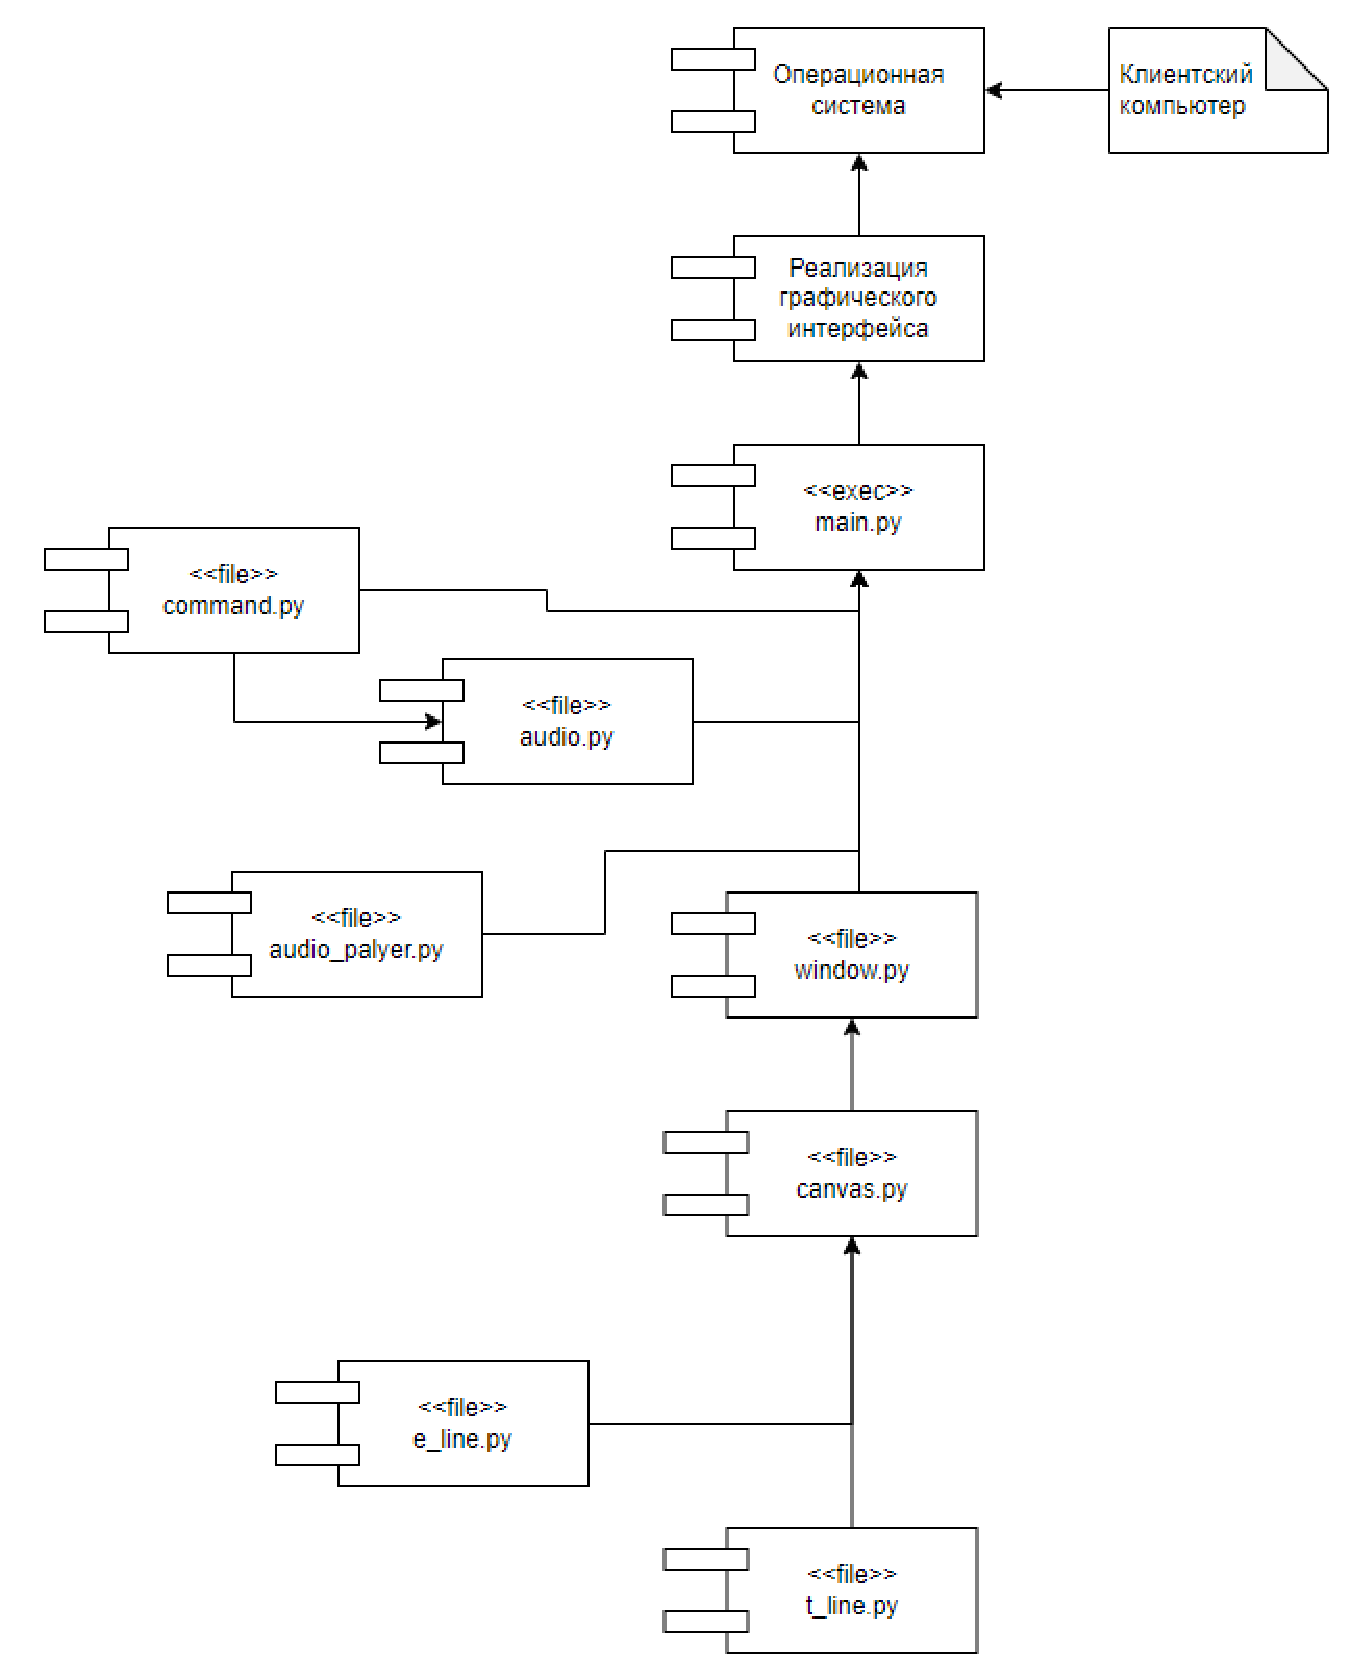
\includegraphics[width=0.7\linewidth]{diagram_comp}}
	\caption{Диаграмма компонентов}
	\label{diagram_comp:image}
\end{figure}

Основным исполняемым файлов является файл main.py, объединяющий в себе все другие компоненты. При запуске происходит создание графичексого интерфейса, посредством которого пользователь может взаимодействовать с программой. 

\subsection{Содержание информационных блоков. Основные сущности}

Проанализировав требования, можно выделить 5 основных сущностей:
\begin{itemize}
	\item "<Аудио">;
	\item "<Аудиоплеер">;
	\item "<Окно">;
	\item "<Холст">;
	\item "<Команда">.
\end{itemize}

Ниже представлены таблицы составов перечисленных выше сущностей.

\begin{xltabular}{\textwidth}{|p{2.1cm}|p{2cm}|l|X|}
	\caption{Атрибуты сущности "<Аудио">}\\ \hline
	\label{news:table}
	\thead{Поле} & \thead{Тип} & \thead{Начальное значение} & \thead{Описание} \\ \hline
	\thead 1 & \thead 2 & \thead 3 & \thead 4 \\ \hline
	\endfirsthead
	\continuecaption{Продолжение таблицы \ref{news:table}}
	\thead 1 & \thead 2 & \thead 3 & \thead 4 \\ \hline
	\finishhead
	nchannels & Integer & 0 & Количество каналов \\ \hline 
	sampwidth & Integer & 0 & Размер сэмплов \\ \hline 
	framerate & Integer & 0 & Частота сэмплов \\ \hline 
	nframes & Integer & 0 & Количество сэмплов \\ \hline 
	comptype & String & NONE & Тип сжатия \\ \hline 
	compname & String & not compressed & Название сжатия \\ \hline 
	chunksize & Integer & 0 & Размер буфера за ед. времени \\ \hline 
	copy buffer & Numpy. array & Numpy.array([], dtype=int16) & Буфер для хранения скопированной области \\ \hline 
	signals data & Numpy. array & Numpy.array([], dtype=int16) & Буфер для хранения прочитанных сэмплов \\ \hline 
	duration & Float & 0.0 & Длительность
\end{xltabular}

\begin{xltabular}{\textwidth}{|p{2cm}|p{2cm}|l|X|}
	\caption{Атрибуты сущности "<Аудиоплеер">}\\ \hline
	\label{news2:table}
	\thead{Поле} & \thead{Тип} & \thead{Начальное значение} & \thead{Описание} \\ \hline
	\thead 1 & \thead 2 & \thead 3 & \thead 4 \\ \hline
	\endfirsthead
	\continuecaption{Продолжение таблицы \ref{news2:table}}
	\thead 1 & \thead 2 & \thead 3 & \thead 4 \\ \hline
	\finishhead
	audio & Audio & Audio(kwargs) & Объект класса Audio \\ \hline 
	bactive & Bool & False & Флаг для проверки активности \\ \hline 
	bplaying & Bool & False & Флаг для проверки проигрывания \\ \hline 
	chunk & Bytes & Пустрокая строка байтов & Проигрываемый аудиобуфер \\ \hline 
	volume & Integer & 100 & Громкость \\ \hline 
	start & Float & 0.0 & Время начала выбранной области \\ \hline 
	start index & Integer & 0 & Индекс начала выбранной области в буфере \\ \hline 
	end & Float & 0.0 & Время конца выбранной области \\ \hline 
	end index & Integer & 0 & Индекс конца выбранной области в буфере \\ \hline 
	current & Float & 0.0 & Время проигрывания
\end{xltabular}

\begin{xltabular}{\textwidth}{|p{2cm}|p{2cm}|l|X|}
	\caption{Атрибуты сущности "<Окно">}\\ \hline
	\label{news3:table}
	\thead{Поле} & \thead{Тип} & \thead{Начальное значение} & \thead{Описание} \\ \hline
	\thead 1 & \thead 2 & \thead 3 & \thead 4 \\ \hline
	\endfirsthead
	\continuecaption{Продолжение таблицы \ref{news3:table}}
	\thead 1 & \thead 2 & \thead 3 & \thead 4 \\ \hline
	\finishhead
	scrollbar & Scrollbar & Scrollbar (kwargs) & Ползунок для просмотра дорожки \\ \hline 
	canvas & Canvas & Canvas(kwargs) & Вспомагательный холст \\ \hline 
	scrollable frame & Frame & Frame(kwargs) & Вспомагательная прокручиваемая рамка \\ \hline 
	scrollable canvas & Scrollable Canvas() & Scrollable Canvas(kwargs) & Прокручиваемый холст \\ \hline 
	frame & Frame & Frame(kwargs) & Главная рамка
\end{xltabular}

\begin{xltabular}{\textwidth}{|p{2cm}|p{2cm}|l|X|}
	\caption{Атрибуты сущности "<Холст">}\\ \hline
	\label{news4:table}
	\thead{Поле} & \thead{Тип} & \thead{Начальное значение} & \thead{Описание} \\ \hline
	\thead 1 & \thead 2 & \thead 3 & \thead 4 \\ \hline
	\endfirsthead
	\continuecaption{Продолжение таблицы \ref{news4:table}}
	\thead 1 & \thead 2 & \thead 3 & \thead 4 \\ \hline
	\finishhead
	loaded & Bool & False & Флаг для проверки загрузки холста \\ \hline 
	player & AudioPla- yer & AudioPlayer(kwargs) & Объект класса AudioPlayer \\ \hline 
	signals & List & [] & Группированные значения амплитуд \\ \hline 
	signals count & Integer & 1 & Количество линий холста \\ \hline 
	pixels per second & Integer & 12 & Количество пикселей, необходимое для отображения 1 секунды звука \\ \hline 
	bdrawing & Bool & False & Флаг для проверки отрисовки \\ \hline 
	block & Bool & False & Флаг для блокировки границ \\ \hline 
	s line & EdgeLine & EdgeLine(kwargs) & Граница начала области \\ \hline 
	e line & EdgeLine & EdgeLine(kwargs) & Граница конца области \\ \hline 
	t line & TimeLine & TimeLine(kwargs) & Линия времени \\ \hline 
	labels & List & [0, [Label()]] & Временные отметки
\end{xltabular}

\begin{xltabular}{\textwidth}{|p{2cm}|p{2cm}|l|X|}
	\caption{Атрибуты сущности "<Команда">}\\ \hline
	\label{news5:table}
	\thead{Поле} & \thead{Тип} & \thead{Начальное значение} & \thead{Описание} \\ \hline
	\thead 1 & \thead 2 & \thead 3 & \thead 4 \\ \hline
	\endfirsthead
	\continuecaption{Продолжение таблицы \ref{news5:table}}
	\thead 1 & \thead 2 & \thead 3 & \thead 4 \\ \hline
	\finishhead
	audio & Audio() & Audio(kwargs) & Объект класса Audio \\ \hline 
	start index & Integer & Задается при вызове конструктора & Индекс начала выбранной области в буфере \\ \hline 
	end index & Integer & Задается при вызове конструктора & Индекс конца выбранной области в буфере \\ \hline 
	buffer & Numpy. array() & [] & Неизмененный фрагмент аудио
\end{xltabular}

В системе предусмотрен внутренний механизм связи между разделами и элементами информационных блоков, поэтому введения дополнительных идентификаторов при реализации связей между сущностями не предполагается.

Экземпляры сущностей реализуются в информационных блоках посредством элементов, атрибуты сущности – посредством полей и свойств элемента. 

\ifПрактика{}\else{
   \section{Рабочий проект}
\subsection{Классы, используемые при разработке программы}

Можно выделить следующий список классов и их методов, использованных при разработке программы (таблица \ref{class:table}).

\renewcommand{\arraystretch}{1.0} % уменьшение расстояний до сетки таблицы
\begin{xltabular}{\textwidth}{|X|p{2.8cm}|>{\setlength{\baselineskip}{0.7\baselineskip}}p{4.05cm}|>{\setlength{\baselineskip}{0.7\baselineskip}}p{4.85cm}|}
\caption{Описание классов, используемых в приложении\label{class:table}}\\
\hline \centrow \setlength{\baselineskip}{0.7\baselineskip} Название класса & \centrow \setlength{\baselineskip}{0.7\baselineskip} Модуль, к которому относится класс & \centrow Описание класса & \centrow Методы \\
\hline \centrow 1 & \centrow 2 & \centrow 3 & \centrow 4\\ \hline
\endfirsthead
\caption*{Продолжение таблицы \ref{class:table}}\\
\hline \centrow 1 & \centrow 2 & \centrow 3 & \centrow 4\\ \hline
\finishhead

\hline Window & window.py & Класс графического интерфеса программы & Дополнительные методы отсутствуют\\

\hline Audio & audio.py & Класс для работы с аудиоданными & copy audio(start index, end index) - копирование области в буфер\\

\hline Canvas & canvas.py & Класс для визуализации аудиоданных & change lines position(start, end, xstart, xend, bplay) - смена позиций границ области, set line(event, bend) - перемещение границ области аудио по нажатию, draw(bstart=False, bend=False, btime=False) - отрисовка аудиодорожки, change scale(badd) - смена масштаба, reset lines(bstart, bend, btime) - сброс позииций границ области\\

\hline EdgeLine & eline.py & Класс границы области аудио & change position(x) - смена позиции\\ 

\hline TimeLine & tline.py & Класс линии времени & change position(x) - смена позиции, movement(event) - событие перемещения, set() - смена текста надписи и ее положения\\

\hline AudioPlayer & audioplayer.py & Класс для загрузки, воспроизведения и сохранения аудио & open player() - инициализация плеера SDL, close player() - закрытие плеера SDL, pause audio(event) - прекращение воспроизведения, resume audio(event) - восстановление воспроизведения, set time borders(start, end, bload, bplay) - установка границ области, set time(start, end, bplay) -- установка линии времени, load file(chunksize=2048) -- загрузка аудиофайла, save file() -- сохранение аудиофайла, save file where() -- сохранение аудиофайла с выбором имени и расположения, load chunk(chunk, start idnex, end index, play, loops) -- загрузка аудиоданных в буфер для воспроизведения, play chunk(chunk) -- воспроизведения из буфера аудиоданных\\

\hline CommandBuff- er & command.py & Класс буфера совершенных над аудиоданными операций & add() -- добавление операции в буфер, clean() -- очищение буфера, move() -- перемещение команд в буфере во избежание переполнения\\ 

\hline Command & command.py & Класс команды редактирования аудио & do() -- совершение операции, undo() -- отмена операции\\

\hline CutCommand & audio.py & Наследник класса Command; представляет собой обработку удаления области аудио & do() -- совершение операции, undo() -- отмена операции\\

\hline PasteCommand & audio.py & Наследник класса Command; представляет собой обработку замены и вставки области в аудио & do() -- совершение операции, undo() -- отмена операции\\

\hline NullifyCom- mand & audio.py & Наследник класса Command; представляет собой обработку обнуления области аудио & do() -- совершение операции, undo() -- отмена операции\\

\hline FadeCommand & audio.py & Наследник класса Command; представляет собой обработку эффекта нарастания и затухания области аудио & do() -- совершение операции, undo() -- отмена операции\\

\hline VolumeCom- mand & audio.py & Наследник класса Command; представляет собой обработку громкости аудио & do() -- совершение операции, undo() -- отмена операции
\end{xltabular}
%\renewcommand{\arraystretch}{1.0} % восстановление сетки

\subsection{Системное тестирование}

Для отладки программы были разработаны следующие тестовые наборы:
	
\subsubsection{Загрузка аудиофайла}
Предусловие: програма запущена.

Тестовый случай: загрузка аудиофайла.
	
Ожидаемый результат: корректная визуализация аудиоданных.

Результат представлен на рисунках \ref{test_case:image} и \ref{test_case1:image}.

\begin{figure}[H]
\center{\includegraphics[width=1\linewidth]{test_case1}}
\caption{Аудиодорожка до загрузки аудиофайла}
\label{test_case:image}
\end{figure}

\begin{figure}[H] 
	\center{\includegraphics[width=1\linewidth]{test_case2}}
	\caption{Аудиодорожка после загрузки аудиофайла}
	\label{test_case1:image}
\end{figure}

\subsubsection{Проигрыввание аудио}
Предусловие: програма запущена, аудиофайл загружен.

Тестовый случай: проигрывание аудио.

Ожидаемый результат: корректное воспроизведение аудиоданных.

Результат представлен на рисунках \ref{test_case2:image} и \ref{test_case3:image}.

\begin{figure}[H]
	\center{\includegraphics[width=1\linewidth]{test_case2}}
	\caption{Аудиодорожка до воспроизведения аудиофайла}
	\label{test_case2:image}
\end{figure}

\begin{figure}[H] 
	\center{\includegraphics[width=1\linewidth]{test_case3}}
	\caption{Аудиодорожка после воспроизведения аудиофайла}
	\label{test_case3:image}
\end{figure}

\subsubsection{Выделение области}
Предусловие: програма запущена, аудиофайл загружен.

Тестовый случай: выделение области аудио.

Ожидаемый результат: корректное выделение области.

Результат представлен на рисунках \ref{test_case5:image} и \ref{test_case6:image}.

\begin{figure}[H]
	\center{\includegraphics[width=1\linewidth]{test_case2}}
	\caption{Аудиодорожка до выбора области}
	\label{test_case5:image}
\end{figure}

\begin{figure}[H] 
	\center{\includegraphics[width=1\linewidth]{test_case4}}
	\caption{Аудиодорожка после выбора области}
	\label{test_case6:image}
\end{figure}

\subsubsection{Редактирование аудиоданных}
Предусловие: програма запущена, аудиофайл загружен, выбрана необходимая область.

Тестовый случай: удаление области.

Ожидаемый результат: корректное удаление области.

Результат представлен на рисунках \ref{test_case7:image} и \ref{test_case8:image}.

\begin{figure}[H]
	\center{\includegraphics[width=1\linewidth]{test_case5}}
	\caption{Аудиодорожка до удаления области}
	\label{test_case7:image}
\end{figure}

\begin{figure}[H] 
	\center{\includegraphics[width=1\linewidth]{test_case6}}
	\caption{Аудиодорожка после удаления области}
	\label{test_case8:image}
\end{figure}

Предусловие: програма запущена, аудиофайл загружен, скопирована вставляемая область.

Тестовый случай: вставка области.

Ожидаемый результат: корректная вставка области.

Результат представлен на рисунках \ref{test_case9:image} и \ref{test_case10:image}.

\begin{figure}[H]
	\center{\includegraphics[width=1\linewidth]{test_case5}}
	\caption{Аудиодорожка до вставки области}
	\label{test_case9:image}
\end{figure}

\begin{figure}[H] 
	\center{\includegraphics[width=1\linewidth]{test_case7}}
	\caption{Аудиодорожка после вставки области}
	\label{test_case10:image}
\end{figure}

Предусловие: програма запущена, аудиофайл загружен, скопирована замещающая и выбрана заменяемая области.

Тестовый случай: вставка области.

Ожидаемый результат: корректная замена области.

Результат представлен на рисунках \ref{test_case11:image} и \ref{test_case12:image}.

\begin{figure}[H]
	\center{\includegraphics[width=1\linewidth]{test_case5}}
	\caption{Аудиодорожка до замены области}
	\label{test_case11:image}
\end{figure}

\begin{figure}[H] 
	\center{\includegraphics[width=1\linewidth]{test_case8}}
	\caption{Аудиодорожка после замены области}
	\label{test_case12:image}
\end{figure}

Предусловие: програма запущена, аудиофайл загружен, выбрана необходимая область.

Тестовый случай: обнуление области.

Ожидаемый результат: корректное обнуление области.

Результат представлен на рисунках \ref{test_case13:image} и \ref{test_case14:image}.

\begin{figure}[H]
	\center{\includegraphics[width=1\linewidth]{test_case5}}
	\caption{Аудиодорожка до обнуления области}
	\label{test_case13:image}
\end{figure}

\begin{figure}[H] 
	\center{\includegraphics[width=1\linewidth]{test_case9}}
	\caption{Аудиодорожка после обнуления области}
	\label{test_case14:image}
\end{figure}

Предусловие: програма запущена, аудиофайл загружен, выбрана необходимая область.

Тестовый случай: нарастание области.

Ожидаемый результат: корректное применение эффекта нарастания области.

Результат представлен на рисунках \ref{test_case15:image} и \ref{test_case16:image}.

\begin{figure}[H]
	\center{\includegraphics[width=1\linewidth]{test_case5}}
	\caption{Аудиодорожка до применения эффекта}
	\label{test_case15:image}
\end{figure}

\begin{figure}[H] 
	\center{\includegraphics[width=1\linewidth]{test_case10}}
	\caption{Аудиодорожка после применения эффекта}
	\label{test_case16:image}
\end{figure}

Предусловие: програма запущена, аудиофайл загружен, выбрана необходимая область.

Тестовый случай: затухание области.

Ожидаемый результат: корректное применение эффекта затухания области.

Результат представлен на рисунках \ref{test_case17:image} и \ref{test_case18:image}.

\begin{figure}[H]
	\center{\includegraphics[width=1\linewidth]{test_case5}}
	\caption{Аудиодорожка до применения эффекта}
	\label{test_case17:image}
\end{figure}

\begin{figure}[H] 
	\center{\includegraphics[width=1\linewidth]{test_case11}}
	\caption{Аудиодорожка после применения эффекта}
	\label{test_case18:image}
\end{figure}

\subsubsection{Управление действиями}

Предусловие: програма запущена, аудиофайл загружен, совершенно какое-либо изменение аудиоданных.

Тестовый случай: отмена операции.

Ожидаемый результат:  корректная отмена совершенной операции.

Результат представлен на рисунках \ref{test_case19:image} и \ref{test_case20:image}.

\begin{figure}[H]
	\center{\includegraphics[width=1\linewidth]{test_case11}}
	\caption{Аудиодорожка до отмены операции}
	\label{test_case19:image}
\end{figure}

\begin{figure}[H] 
	\center{\includegraphics[width=1\linewidth]{test_case2}}
	\caption{Аудиодорожка после отмены операции}
	\label{test_case20:image}
\end{figure}

Предусловие: програма запущена, аудиофайл загружен, совершенно какое-либо изменение аудиоданных.

Тестовый случай: возврат операции.

Ожидаемый результат: корректный возврат совершенной операции.

Результат представлен на рисунках \ref{test_case21:image} и \ref{test_case22:image}.

\begin{figure}[H]
	\center{\includegraphics[width=1\linewidth]{test_case2}}
	\caption{Аудиодорожка до возврата операции}
	\label{test_case21:image}
\end{figure}

\begin{figure}[H] 
	\center{\includegraphics[width=1\linewidth]{test_case11}}
	\caption{Аудиодорожка после возврата операции}
	\label{test_case22:image}
\end{figure}

\subsubsection{Сохранение аудиофайла}

Предусловие: програма запущена, аудиофайл загружен, совершенны какие-либо операции над аудиоданными (необязательно).

Тестовый случай: сохранение аудиофайла.

Ожидаемый результат: корректное сохранение аудиофайла.

Результат представлен на рисунках \ref{test_case23:image} и \ref{test_case24:image}.

\begin{figure}[H]
	\center{\includegraphics[width=0.5\linewidth]{test_case12}}
	\caption{Размер оригинального аудиофайла}
	\label{test_case23:image}
\end{figure}

\begin{figure}[H] 
	\center{\includegraphics[width=0.5\linewidth]{test_case13}}
	\caption{Размер аудиофайла после сохранения с изменениями}
	\label{test_case24:image}
\end{figure}
   \section*{ЗАКЛЮЧЕНИЕ}
\addcontentsline{toc}{section}{ЗАКЛЮЧЕНИЕ}

Современный мир музыки и звукозаписи не может обойтись без аудиоредакторов. Они стали незаменимыми инструментами в музыкальной индустрии, радиовещании, телевидении, видеопроизводстве, кино и других областях, где необходимо обрабатывать и улучшать звуковые файлы. Соответственно, профессиональные навыки работы с аудиоредакторами являются очень актуальными на современном рынке труда. Владение компьютерными программами для звукозаписи и редактирования аудиофайлов открывает широкие возможности для работы в медиа-индустрии и музыкальном бизнесе. Кроме этого, возможности аудиоредакторов легко доступны и для любителей – они могут использоваться для создания и обработки интересных и креативных музыкальных проектов.


Основные результаты работы:

\begin{enumerate}
\item Проведен анализ предметной области.
\item Разработана концептуальная модель программы.
\item Разработана архитектура программы.
\item Реализован пользовательский интерфейс.
\item Проведено системное тестирование.
\end{enumerate}

Все требования, объявленные в техническом задании, были полностью реализованы, все задачи, поставленные в начале разработки проекта, были также решены.

Готовый рабочий проект представлен программой расширения .exe.

}\fi
\addcontentsline{toc}{section}{СПИСОК ИСПОЛЬЗОВАННЫХ ИСТОЧНИКОВ}

\begin{thebibliography}{9}

    \bibitem{1} Лерч А. "Python для анализа звука" / Александр Лерч. – Packt Publishing, 2013. – 504 с. – ISBN: 978-1-78216-889-6. – Текст: непосредственный.
    \bibitem{2} Бек Э. "Python для музыкального программирования" / Эндрю Бек. – Course Technology PTR, 2008. – 351 с. – ISBN: 978-1-59863-601-9. – Текст: непосредственный.
    \bibitem{3} Рид М. "Обработка звука в Python" / Майк Рид. – CreateSpace Independent Publishing Platform, 2015. – 286 с. – ISBN: 978-1-5177-1464-8. – Текст: непосредственный.
    \bibitem{4}	Бильбао С. "Python Sound: обработка сигналов и акустика" / Стефан Бильбао. – CRC Press, 2018. – 454 с. – ISBN: 978-0-367-19283-3. – Текст: непосредственный.
	\bibitem{5} Мэнк Дж. "Python для обработки аудиосигналов" / Джозеф Мэнк. – Springer, 2015. – 426 с. – ISBN: 978-3-319-21947-8. – Текст: непосредственный.
	\bibitem{6}	Гвидо ван Россум. "Python: основы программирования" / Гвидо ван Россум. – Москва: ДМК Пресс, 2019. – 232 с. – ISBN: 978-5-97060-762-7. – Текст: непосредственный.
	\bibitem{7}	Маннинг С. "Python машинного обучения: Сборник рецептов" / Стивен Маннинг. - SPb.: Питер, 2018. - 384 с. - ISBN: 978-5-4461-0598-9. - Текст: непосредственный.
	\bibitem{8} Миллер М. "Учимся писать игры на Python" / Майк Миллер. - М.: ДМК Пресс, 2018. - 320 с. - ISBN: 978-5-97060-560-9. - Текст: непосредственный.
	\bibitem{9} Златопольский Д.М. "Python. Курс основного уровня" / Златопольский Д.М. - СПб.: Питер, 2018. - 400 с. - ISBN: 978-5-496-02465-5. - Текст: непосредственный.   
%	\bibitem{10} Рейд К. "Python для детей и самых начинающих" / Келли Рейд. - М.: ДМК Пресс, 2020. - 336 с. - ISBN: 978-5-6043407-8-2. - Текст: непосредственный.
	\bibitem{10} Мартелли А. "Python в примерах: учебное пособие" / Алекс Мартелли, Дэвид Гудгертьс, Идан Газит. - М.: ДМК Пресс, 2018. - 616 с. - ISBN: 978-5-97060-533-3. - Текст: непосредственный.
	\bibitem{11} ВандерПлас Дж. "Python для анализа данных" / Джейк ВандерПлас. - М.: ДМК Пресс, 2018. - 592 с. - ISBN: 978-5-97060-279-0. - Текст: непосредственный.
\end{thebibliography}

\ifВКР{\input{Плакаты}}\fi
\ifПрактика{}\else{\appendix{Фрагменты исходного кода программы}

main.py
\lstinputlisting[language=Python, frame=none]{main.py}
\newpage

audio.py
\lstinputlisting[language=Python, frame=none]{audio.py}
\newpage

audioplayer.py
\lstinputlisting[language=Python, frame=none]{audioplayer.py}}\fi
\end{document}
